\subsubsection{The addaccu circuit}

\begin{figure}[h!]
\centering
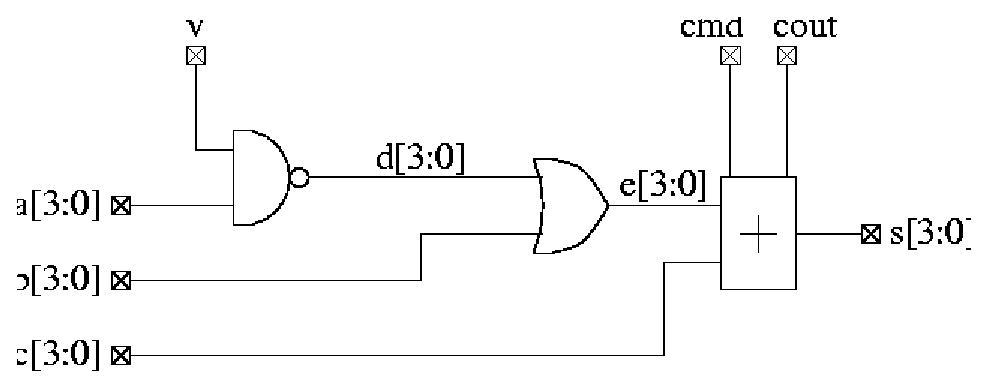
\includegraphics[width=.9\textwidth]{./images/add1}
\end{figure}
  
\newpage
\subsubsection{The data-path}

\begin{figure}[h!]
\centering
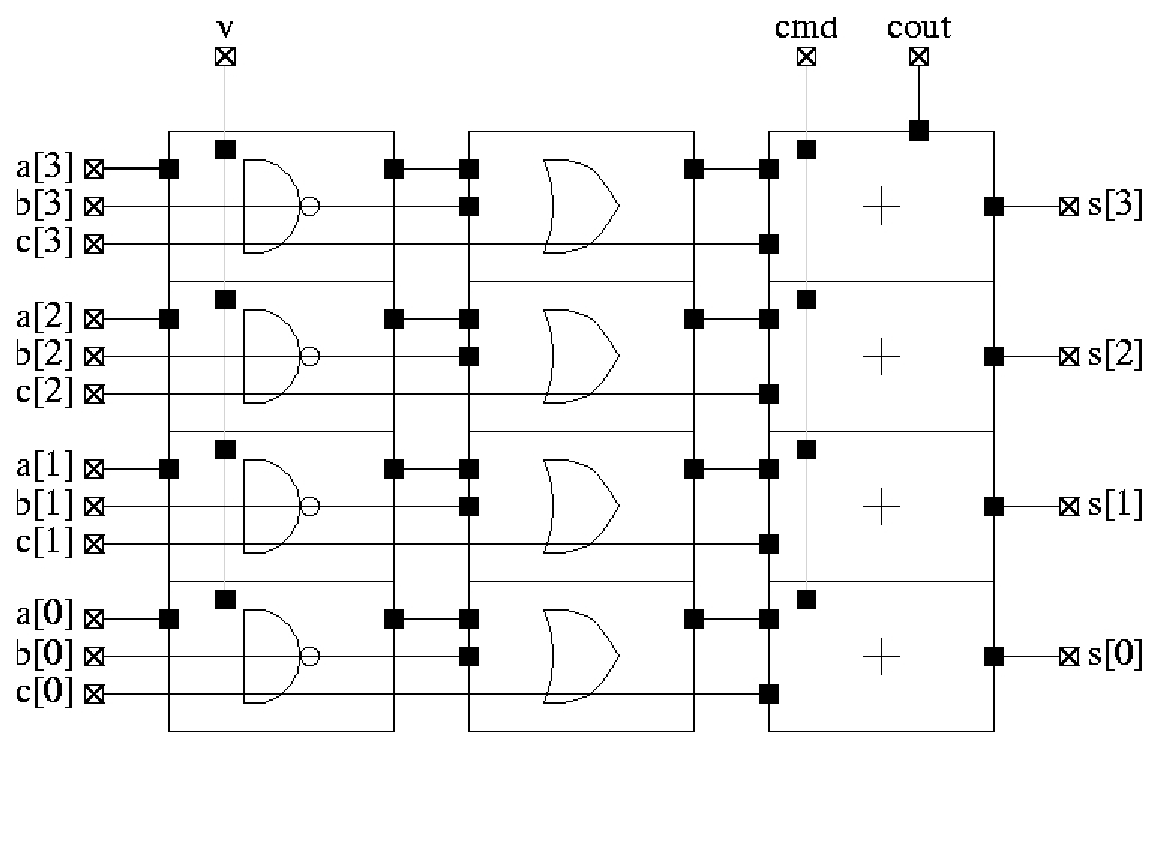
\includegraphics[width=.9\textwidth]{./images/add2}
\end{figure}

\newpage
\subsubsection{Description of the circuit with \emph{Stratus} : file addaccu.py}

\begin{figure}[h!]
\centering
\includegraphics[width=1.4\textwidth]{./images/addaccu1}
\end{figure}

\begin{figure}[h!]
\centering
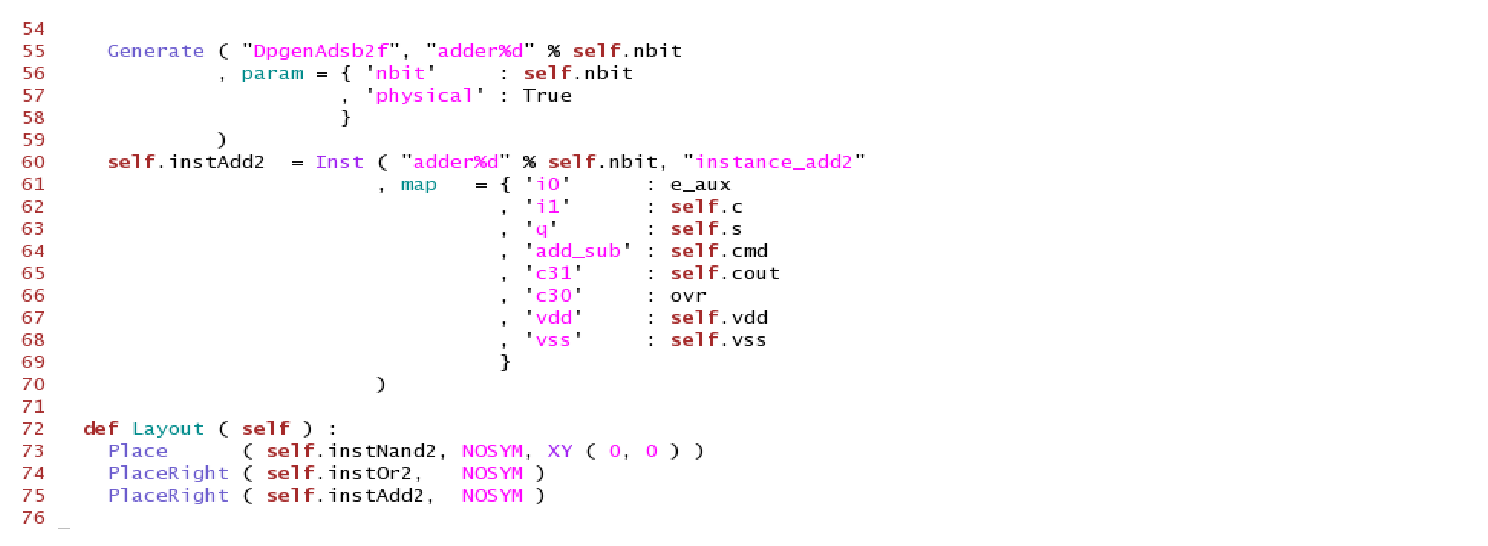
\includegraphics[width=1.4\textwidth]{./images/addaccu2}
\end{figure}

\newpage
\subsubsection{Creation of the circuit : file test.py}

\begin{figure}[h!]
\centering
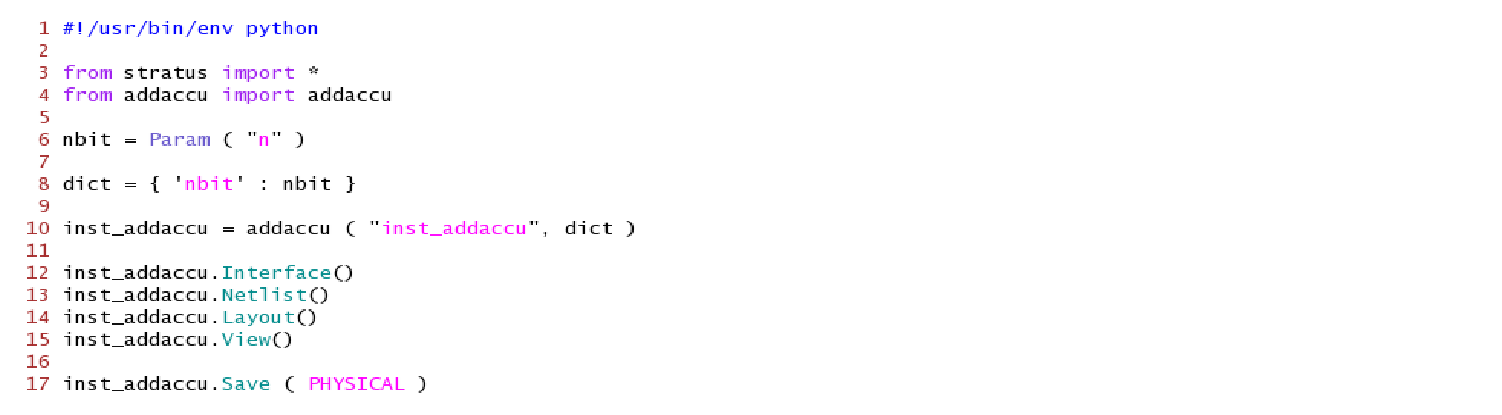
\includegraphics[width=1.4\textwidth]{./images/test}
\end{figure}

\subsubsection{How to execute the file}

\begin{verbatim}
python test.py -n 4
\end{verbatim}
\indent or :
\begin{verbatim}
chmod u+x test.py
./test -n 4
\end{verbatim}

\subsubsection{The editor}

The method \verb-View- permits to open an editor in which one can see the cell being created as shown in the picture below.
\begin{figure}[h!]
\centering
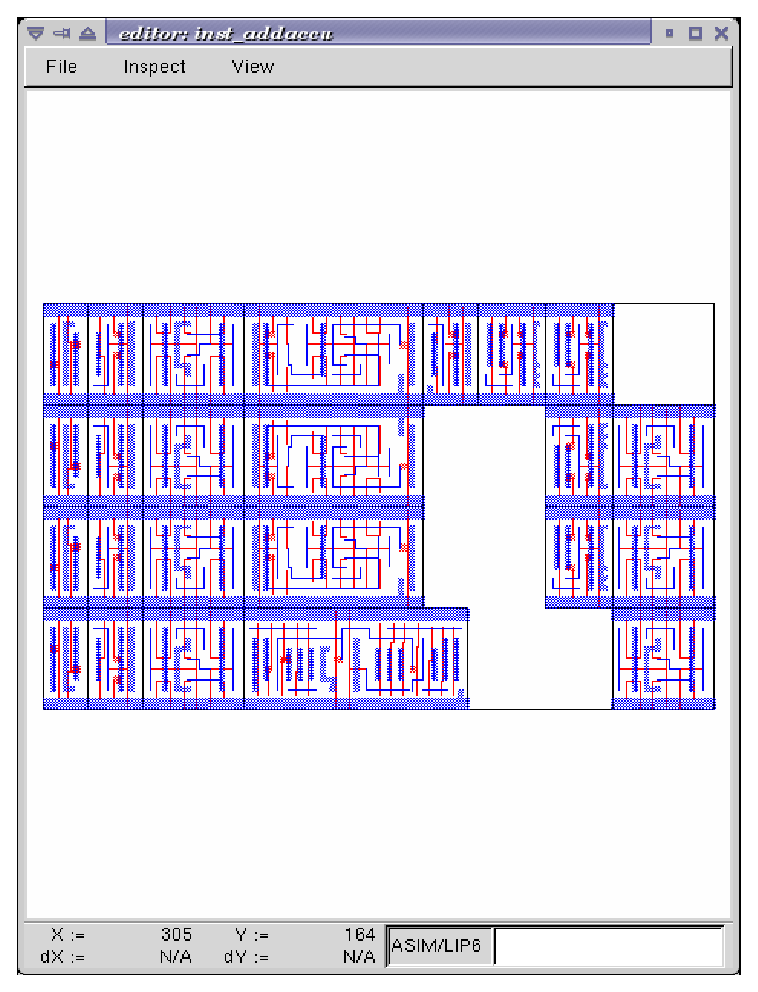
\includegraphics[width=.8\textwidth]{./images/editor}
\end{figure}

\newpage
\subsubsection{Function Param}

This function allows the user to give parameters when creating a cell.\\
\indent When one wants to give values to two parameters, one can type on the shell :
\begin{verbatim}
python test.py -n 4 -w 8
\end{verbatim}
\indent The file \verb-test.py- has then to contain :
\begin{verbatim}
nbit, nword = Param ( "n", "w" )
\end{verbatim}
\indent The letters typed on the shell must be the ones given as parameters of function \verb-Param-.

\subsubsection{How to instanciate your generator in another generator}

One can create a generator and instantiate it in another generator.\\
\indent To do that, the model name of the generator must have the form : "file\_name.class\_name".\\    
\indent Note that if the two generators are not in the same directory, the directory of the generator to be instantiated has to be added in the CRL\_CATA\_LIB environment variable.\\

\indent For example, in order to instanciate the addaccu created above in a cell :
\begin{verbatim}
n = 4
Generate ( "addaccu.addaccu", "my_addaccu_%dbits" % n
         , param = { 'nbit' : n } )

Inst ( "my_addaccu_%dbits" % n
     , map = { 'a'    : self.netA
             , 'b'    : self.netB
             , 'c'    : self.netC
             , 'v'    : self.netV
             , 'cmd'  : self.netCmd
             , 'cout' : self.netCout
             , 's'    : self.netS
             , 'vdd'  : self.vdd
             , 'vss'  : self.vss
             }
     )
\end{verbatim}

\begin{htmlonly}

\subsubsection{See Also}

\hyperref[ref]{\emph{Introduction}}{}{Introduction}{secintroduction}
\hyperref[ref]{\emph{Netlist}}{}{Netlist}{secnetlist}
\hyperref[ref]{\emph{Layout}}{}{Layout}{seclayout}
\hyperref[ref]{\emph{Place and Route}}{}{Place and Route}{secroute}
\hyperref[ref]{\emph{Virtual libraty}}{}{Virtual library}{seclibrary}
\hyperref[ref]{\emph{Instanciation facilities}}{}{Instanciation facilities}{secfacilities}

\end{htmlonly}
